% Concise architecture figure of M1 (1 page). Detailed version: hinh_kien_truc_M1.tex.
% Compile: pdflatex (Overleaf: pdfLaTeX).
\documentclass[tikz,border=8pt]{standalone}
\usepackage{amsmath,amssymb}
\usetikzlibrary{positioning,arrows.meta,calc}

\tikzset{
  >={Stealth[length=2mm]},
  qbox/.style={draw=blue!60!black, fill=blue!9, rounded corners=2pt, align=center, font=\small, inner sep=4pt},
  cbox/.style={draw=orange!75!black, fill=orange!13, rounded corners=2pt, align=center, font=\small, inner sep=4pt},
  dbox/.style={draw=black!55, fill=black!4, rounded corners=2pt, align=center, font=\small, inner sep=4pt},
  flow/.style={->, thick, black!70},
}

\begin{document}
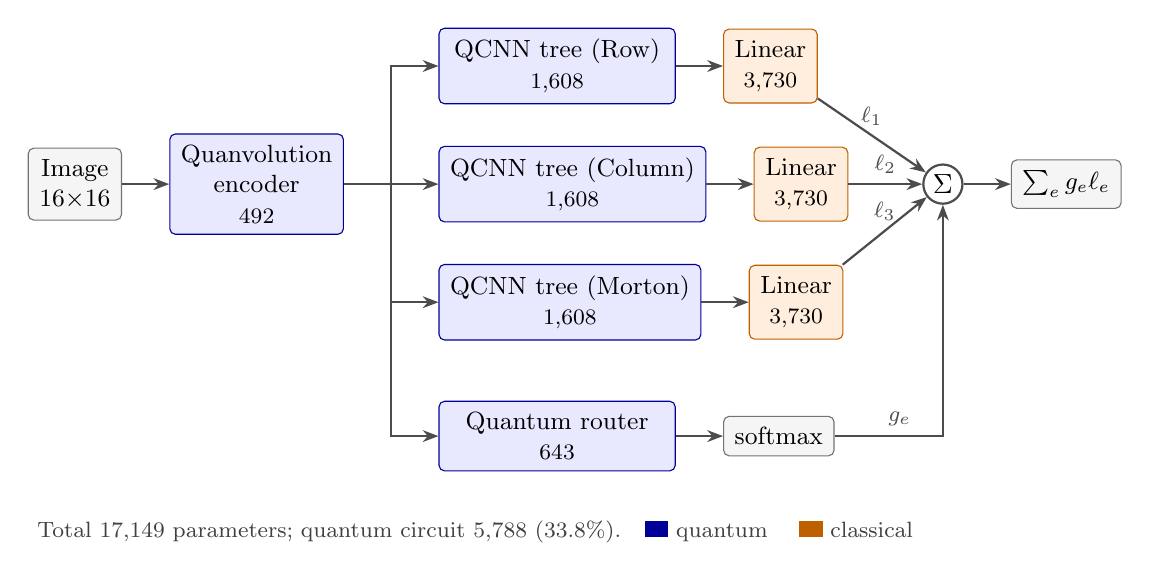
\begin{tikzpicture}

  \node[dbox] (in) at (0,0) {Image\\$16{\times}16$};
  \node[qbox, right=6mm of in] (enc) {Quanvolution\\encoder\\\footnotesize 492};

  \coordinate (sp) at ($(enc.east)+(6mm,0)$);
  \foreach \name/\lab/\y in {t0/Row/1.5, t1/Column/0, t2/Morton/-1.5} {
    \node[qbox, anchor=west, minimum width=30mm] (\name) at ($(sp)+(6mm,\y)$) {QCNN tree (\lab)\\\footnotesize 1{,}608};
  }
  \foreach \name/\i in {t0/1, t1/2, t2/3} {
    \node[cbox, right=6mm of \name] (h\i) {Linear\\\footnotesize 3{,}730};
    \draw[flow] (\name) -- (h\i);
  }
  \node[qbox, anchor=west, minimum width=30mm] (rt) at ($(sp)+(6mm,-3.2)$) {Quantum router\\\footnotesize 643};
  \node[dbox, right=6mm of rt] (sm) {softmax};
  \draw[flow] (rt) -- (sm);

  \node[draw=black!70, circle, thick, inner sep=1.5pt] (mix) at ($(h2.east)+(12mm,0)$) {$\Sigma$};
  \foreach \i in {1,2,3} { \draw[flow] (h\i) -- node[above, font=\footnotesize] {$\ell_{\i}$} (mix); }
  \draw[flow] (sm.east) -| node[pos=0.3, above, font=\footnotesize] {$g_e$} (mix.south);
  \node[dbox, right=6mm of mix] (out) {$\sum_e g_e \ell_e$};
  \draw[flow] (mix) -- (out);

  \draw[flow] (in) -- (enc);
  \draw[thick, black!70] (enc.east) -- (sp);
  \foreach \name in {t0,t1,t2,rt} { \draw[flow] (sp) |- (\name.west); }

  \node[font=\footnotesize, text=black!75, anchor=north west] at ($(in.west |- rt.south)+(0,-5mm)$) {%
    Total 17{,}149 parameters; quantum circuit 5{,}788 (33.8\%).\quad
    \textcolor{blue!60!black}{\rule{3mm}{2mm}} quantum \quad \textcolor{orange!75!black}{\rule{3mm}{2mm}} classical};
\end{tikzpicture}
\end{document}
